\documentclass[11pt]{article}

\usepackage{fancyvrb}
\usepackage{tikz}
\usetikzlibrary{shapes}
\usepackage[empty]{fullpage}

\begin{document}
\section*{Project 3 \hfill CS 261}

\textit{Save your program for this project as} \verb|<emailID>_project3.py| \textit{where} \verb|<emailID>| \textit{is the part of your Hampden-Sydney e-mail address before the @ symbol. When you are finished, e-mail your program to} \verb|blins@hsc.edu|. \textit{Your solution is due by noon on Friday, September 20. }

\subsection*{Binary Representation of Decimals}

Floating point errors happen because floating point numbers are stored in base-2, which isn't a perfect match for our number system.  For example, in Python 

\begin{verbatim}
>>> 0.1 + 0.1 + 0.1
0.30000000000000004
\end{verbatim}

\noindent
In this project we will implement an algorithm to convert any nonnegative floating point number $x$ that is less than 1 into a string of ones and zeros that represents its binary decimal form.  A flow chart for the algorithm is shown below.  



\begin{center}

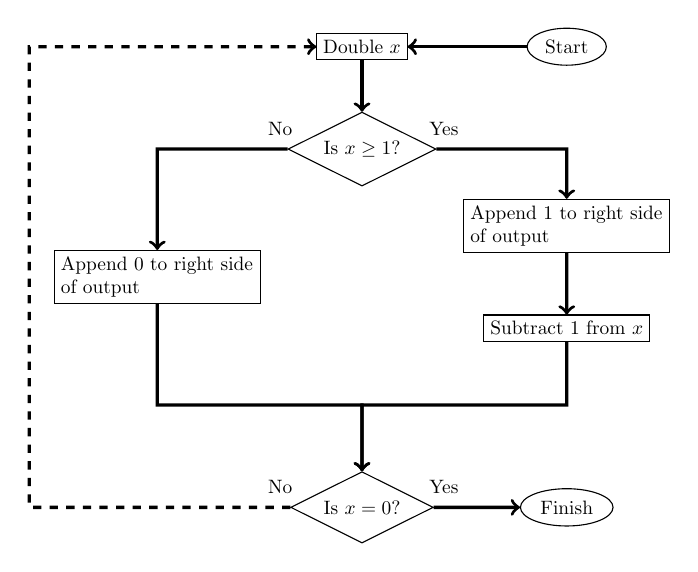
\begin{tikzpicture}[scale=0.65]
\node[scale=0.7,draw=black, ellipse] (S) at (4, 0)  {Start}; 
\node[scale=0.7,draw=black, rectangle] (A) at (0, 0)  {Double $x$}; 
\node[scale=0.7,draw=black, diamond, shape aspect=2] (B) at (0,-2)  {Is $x \ge 1$?}; 
\node[scale=0.7,draw=black, rectangle, text width=3.5cm] (C) at (4,-3.5)  {Append 1 to right side of output}; 
\node[scale=0.7,draw=black, rectangle, text width=3.5cm] (D) at (-4,-4.5)  {Append 0 to right side of output}; 
\node[scale=0.7,draw=black, rectangle] (E) at (+4,-5.5)  {Subtract 1 from $x$}; 
\node[scale=0.7,draw=black, diamond, shape aspect=2] (F) at (0,-9)  {Is $x = 0$?}; 
\node[scale=0.7,draw=black, ellipse] (G) at (4,-9)  {Finish}; 
\draw[very thick, ->] (S) -- (A);
\draw[very thick, ->] (A) -- (B);
\draw[very thick, ->] (B) -- (+4,-2) -- (C);
\draw[very thick, ->] (B) -- (-4,-2) -- (D);
\draw[very thick, ->] (C) -- (E);
\draw[very thick, ->] (D) -- (-4,-7) -- (0,-7) -- (F);
\draw[very thick, ->] (E) -- (+4,-7) -- (0,-7) -- (F);
\draw[very thick, ->] (F) -- (G);
\draw[very thick, dashed, ->] (F) -- (-6.5,-9) -- (-6.5,0) -- (A);
\draw (1.6,-1.6) node[scale=0.7]  {Yes};
\draw (-1.6,-1.6) node[scale=0.7]  {No};
\draw (1.6,-8.6) node[scale=0.7]  {Yes};
\draw (-1.6,-8.6) node[scale=0.7]  {No};
\end{tikzpicture}

\end{center}

\begin{enumerate}
\item Write a function called \verb|decimal_to_binary(x)| to implement this algorithm.

\item This algorithm will run forever for most inputs. Your function should have some way to prevent this and eventually print out at least the first 10 digits if the binary string doesn't terminate. %Add a constant \verb|MAX_OUTPUT_SIZE|.  Have the function terminate whenever the output length reaches \verb|MAX_OUTPUT_SIZE|.  

\item Test your function on these examples. 
\begin{verbatim}
decimal_to_binary(0.75) # should get 0.11
decimal_to_binary(0.1)  # should get 0.0001100110 
\end{verbatim}

\item Use a similar algorithm to create a function \verb|decimal_to_ternary(x)| that converts $x$ to a ternary (base-3) string. 
\begin{verbatim}
decimal_to_ternary(0.5)  # should get 0.1111111111
decimal_to_ternary(0.25) # should get 0.0202020202 
\end{verbatim}
To adjust the old algorithm, you'll need to triple $x$ at each stage, and then there will be three possibilities: if $x \ge 2$, if $2 > x \ge 1$, and $x < 1$.  
\end{enumerate}


\end{document}
